\section{Docker}

Docker to platforma wirtualizacyjna, opublikowana przez firmę Docker, Inc. w marcu 2013 roku \cite{archiveDotCloudAbout}, która umożliwia tworzenie, uruchamianie oraz zarządzanie kontenerami aplikacji \cite{dockerHome}. 
Kontenery są izolowanymi jednostkami oprogramowania, które zawierają wszystkie niezbędne zależności oraz środowisko uruchomieniowe potrzebne do poprawnego działania aplikacji.
Docker wykorzystuje technologię konteneryzacji, co pozwala na przenośność aplikacji między różnymi środowiskami oraz zapewnia spójność działania na różnych platformach.

Jedną z kluczowych cech Dockera jest jego szybkość oraz lekkość.
Kontenery są uruchamiane na poziomie systemu operacyjnego gospodarza, co eliminuje narzut związany z wirtualizacją tradycyjną.
Porównanie architektury maszyny wirtualnej oraz Docker zostało zaprezentowane na rysunku \ref{rys:docker-vs-vm}.

\begin{figure}[!hb]
	\centering 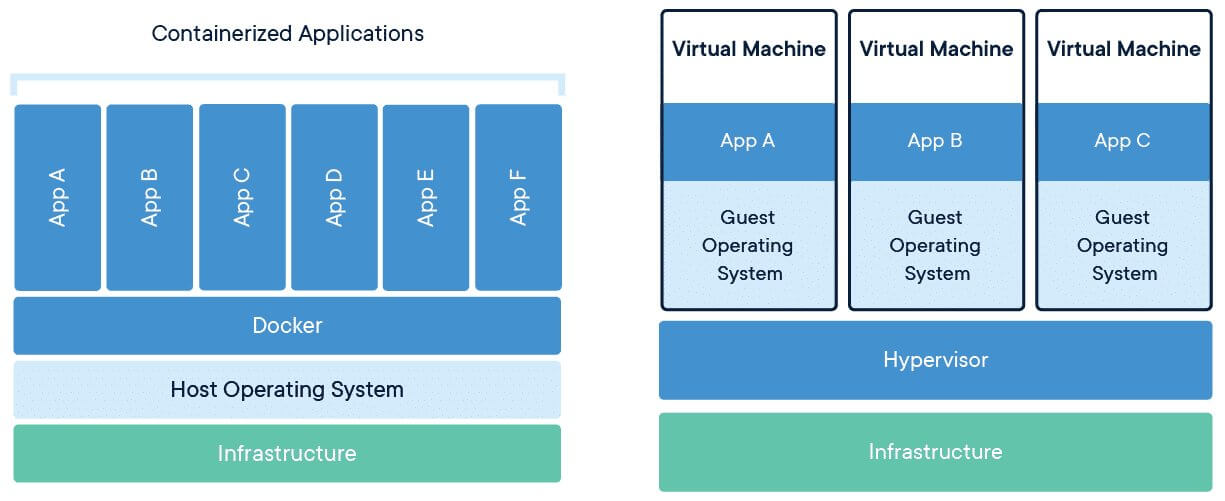
\includegraphics[width=1\linewidth]{rysunki/docker-vs-vm.jpg}
	\caption{Schemat porównania koncepcji maszyny wirtualnej oraz Dockera - źródło \cite{cherryserversOverview}}
	\label{rys:docker-vs-vm}
\end{figure}

Dzięki temu aplikacje uruchomione w kontenerach Docker są bardzo wydajne i mogą być łatwo skalowane w zależności od obciążenia.
Maszyna wirtualna dockerowa nie ma narzutu systemowego na sobie, stąd więcej takich maszyn można uruchomić naraz.

Docker jest również popularnym narzędziem w środowiskach deweloperskich oraz produkcyjnych.
Pozwala on programistom tworzyć odizolowane środowiska programistyczne, co ułatwia testowanie i debugowanie aplikacji.
Jest powszechnie stosowany w procesie wdrażania aplikacji, umożliwiając szybkie i spójne wdrożenie aplikacji na różne serwery oraz platformy chmurowe.
Dzięki wsparciu dla narzędzi takich jak Kubernetes czy Docker Swarm, Docker jest używany do budowy i zarządzania dużymi klastrami kontenerów, co umożliwia elastyczne i skalowalne wdrażanie aplikacji w różnych środowiskach produkcyjnych.

